\documentclass[11pt,letterpaper,]{article}
\usepackage{lmodern}
\usepackage{amssymb,amsmath}
\usepackage{ifxetex,ifluatex}
\usepackage{fixltx2e} % provides \textsubscript
\ifnum 0\ifxetex 1\fi\ifluatex 1\fi=0 % if pdftex
  \usepackage[T1]{fontenc}
  \usepackage[utf8]{inputenc}
\else % if luatex or xelatex
  \ifxetex
    \usepackage{mathspec}
  \else
    \usepackage{fontspec}
  \fi
  \defaultfontfeatures{Ligatures=TeX,Scale=MatchLowercase}
\fi
% use upquote if available, for straight quotes in verbatim environments
\IfFileExists{upquote.sty}{\usepackage{upquote}}{}
% use microtype if available
\IfFileExists{microtype.sty}{%
\usepackage{microtype}
\UseMicrotypeSet[protrusion]{basicmath} % disable protrusion for tt fonts
}{}
\usepackage[margin=1in]{geometry}
\usepackage{hyperref}
\hypersetup{unicode=true,
            pdftitle={A Data Science Lab Project Template in R Markdown},
            pdfauthor={Wenjie Wang},
            pdfkeywords={Template, R Markdown, bookdown, Data Lab},
            pdfborder={0 0 0},
            breaklinks=true}
\urlstyle{same}  % don't use monospace font for urls
\usepackage{natbib}
\bibliographystyle{asa}
\usepackage{color}
\usepackage{fancyvrb}
\newcommand{\VerbBar}{|}
\newcommand{\VERB}{\Verb[commandchars=\\\{\}]}
\DefineVerbatimEnvironment{Highlighting}{Verbatim}{commandchars=\\\{\}}
% Add ',fontsize=\small' for more characters per line
\usepackage{framed}
\definecolor{shadecolor}{RGB}{248,248,248}
\newenvironment{Shaded}{\begin{snugshade}}{\end{snugshade}}
\newcommand{\AlertTok}[1]{\textcolor[rgb]{0.94,0.16,0.16}{#1}}
\newcommand{\AnnotationTok}[1]{\textcolor[rgb]{0.56,0.35,0.01}{\textbf{\textit{#1}}}}
\newcommand{\AttributeTok}[1]{\textcolor[rgb]{0.77,0.63,0.00}{#1}}
\newcommand{\BaseNTok}[1]{\textcolor[rgb]{0.00,0.00,0.81}{#1}}
\newcommand{\BuiltInTok}[1]{#1}
\newcommand{\CharTok}[1]{\textcolor[rgb]{0.31,0.60,0.02}{#1}}
\newcommand{\CommentTok}[1]{\textcolor[rgb]{0.56,0.35,0.01}{\textit{#1}}}
\newcommand{\CommentVarTok}[1]{\textcolor[rgb]{0.56,0.35,0.01}{\textbf{\textit{#1}}}}
\newcommand{\ConstantTok}[1]{\textcolor[rgb]{0.00,0.00,0.00}{#1}}
\newcommand{\ControlFlowTok}[1]{\textcolor[rgb]{0.13,0.29,0.53}{\textbf{#1}}}
\newcommand{\DataTypeTok}[1]{\textcolor[rgb]{0.13,0.29,0.53}{#1}}
\newcommand{\DecValTok}[1]{\textcolor[rgb]{0.00,0.00,0.81}{#1}}
\newcommand{\DocumentationTok}[1]{\textcolor[rgb]{0.56,0.35,0.01}{\textbf{\textit{#1}}}}
\newcommand{\ErrorTok}[1]{\textcolor[rgb]{0.64,0.00,0.00}{\textbf{#1}}}
\newcommand{\ExtensionTok}[1]{#1}
\newcommand{\FloatTok}[1]{\textcolor[rgb]{0.00,0.00,0.81}{#1}}
\newcommand{\FunctionTok}[1]{\textcolor[rgb]{0.00,0.00,0.00}{#1}}
\newcommand{\ImportTok}[1]{#1}
\newcommand{\InformationTok}[1]{\textcolor[rgb]{0.56,0.35,0.01}{\textbf{\textit{#1}}}}
\newcommand{\KeywordTok}[1]{\textcolor[rgb]{0.13,0.29,0.53}{\textbf{#1}}}
\newcommand{\NormalTok}[1]{#1}
\newcommand{\OperatorTok}[1]{\textcolor[rgb]{0.81,0.36,0.00}{\textbf{#1}}}
\newcommand{\OtherTok}[1]{\textcolor[rgb]{0.56,0.35,0.01}{#1}}
\newcommand{\PreprocessorTok}[1]{\textcolor[rgb]{0.56,0.35,0.01}{\textit{#1}}}
\newcommand{\RegionMarkerTok}[1]{#1}
\newcommand{\SpecialCharTok}[1]{\textcolor[rgb]{0.00,0.00,0.00}{#1}}
\newcommand{\SpecialStringTok}[1]{\textcolor[rgb]{0.31,0.60,0.02}{#1}}
\newcommand{\StringTok}[1]{\textcolor[rgb]{0.31,0.60,0.02}{#1}}
\newcommand{\VariableTok}[1]{\textcolor[rgb]{0.00,0.00,0.00}{#1}}
\newcommand{\VerbatimStringTok}[1]{\textcolor[rgb]{0.31,0.60,0.02}{#1}}
\newcommand{\WarningTok}[1]{\textcolor[rgb]{0.56,0.35,0.01}{\textbf{\textit{#1}}}}
\usepackage{longtable,booktabs}
\usepackage{graphicx,grffile}
\makeatletter
\def\maxwidth{\ifdim\Gin@nat@width>\linewidth\linewidth\else\Gin@nat@width\fi}
\def\maxheight{\ifdim\Gin@nat@height>\textheight\textheight\else\Gin@nat@height\fi}
\makeatother
% Scale images if necessary, so that they will not overflow the page
% margins by default, and it is still possible to overwrite the defaults
% using explicit options in \includegraphics[width, height, ...]{}
\setkeys{Gin}{width=\maxwidth,height=\maxheight,keepaspectratio}
\IfFileExists{parskip.sty}{%
\usepackage{parskip}
}{% else
\setlength{\parindent}{0pt}
\setlength{\parskip}{6pt plus 2pt minus 1pt}
}
\setlength{\emergencystretch}{3em}  % prevent overfull lines
\providecommand{\tightlist}{%
  \setlength{\itemsep}{0pt}\setlength{\parskip}{0pt}}
\setcounter{secnumdepth}{5}
% Redefines (sub)paragraphs to behave more like sections
\ifx\paragraph\undefined\else
\let\oldparagraph\paragraph
\renewcommand{\paragraph}[1]{\oldparagraph{#1}\mbox{}}
\fi
\ifx\subparagraph\undefined\else
\let\oldsubparagraph\subparagraph
\renewcommand{\subparagraph}[1]{\oldsubparagraph{#1}\mbox{}}
\fi

%%% Use protect on footnotes to avoid problems with footnotes in titles
\let\rmarkdownfootnote\footnote%
\def\footnote{\protect\rmarkdownfootnote}

%%% Change title format to be more compact
\usepackage{titling}

% Create subtitle command for use in maketitle
\newcommand{\subtitle}[1]{
  \posttitle{
    \begin{center}\large#1\end{center}
    }
}

\setlength{\droptitle}{-2em}

  \title{A Data Science Lab Project Template in R Markdown}
    \pretitle{\vspace{\droptitle}\centering\huge}
  \posttitle{\par}
    \author{Wenjie Wang\footnote{\href{mailto:wenjie.2.wang@uconn.edu}{\nolinkurl{wenjie.2.wang@uconn.edu}};
  Ph.D.~student at Department of Statistics, University of Connecticut.}}
    \preauthor{\centering\large\emph}
  \postauthor{\par}
      \predate{\centering\large\emph}
  \postdate{\par}
    \date{21 September 2018}

\usepackage{booktabs}
\usepackage{amsthm}
\usepackage{amsmath}

\providecommand{\keywords}[1]{\textit{Keywords:} #1}

% consistent with R manual
\newcommand{\pkg}[1]{{\normalfont\fontseries{b}\selectfont #1}}
\let\proglang=\textsf
\let\code=\texttt

\usepackage{amsthm}
\newtheorem{theorem}{Theorem}[section]
\newtheorem{lemma}{Lemma}[section]
\newtheorem{corollary}{Corollary}[section]
\newtheorem{proposition}{Proposition}[section]
\newtheorem{conjecture}{Conjecture}[section]
\theoremstyle{definition}
\newtheorem{definition}{Definition}[section]
\theoremstyle{definition}
\newtheorem{example}{Example}[section]
\theoremstyle{definition}
\newtheorem{exercise}{Exercise}[section]
\theoremstyle{remark}
\newtheorem*{remark}{Remark}
\newtheorem*{solution}{Solution}
\let\BeginKnitrBlock\begin \let\EndKnitrBlock\end
\begin{document}
\maketitle
\begin{abstract}
This is a template mainly designed for data science lab projects. In
this template, we review most common components of a single R Markdown
document with the power of the \textbf{bookdown} package and demonstrate
their basic usage through examples.
\end{abstract}

\keywords{Template; \proglang{R Markdown}; \pkg{bookdown}; \pkg{knitr};
\pkg{Pandoc}}

\hypertarget{l}{%
\section{l}\label{l}}

\[f(x;\theta)=\frac{1}{\pi[1+(x-\theta)^2]}, x\in R, \theta \in R.\]
\begin{equation}
 \begin{split}
&L(\theta)&=\frac{1}{\pi^n \prod_{i=1}^{n}[1+(\theta-X_i)^2]}\\
&\ell(\theta)&=\log(L(\theta))=-\log(\pi^n)-\log(\prod_{i=1}^{n}[1+(\theta-X_i)^2])\\
&&=-n\ln\pi-\sum_{i=1}^{n} \ln[1+(\theta-X_i)^2]\\
&\ell^{\prime} (\theta) &=0-2\sum_{i=1}^{n} \frac {\theta-X_i}{1+(\theta-X_i)^2}=-2\sum_{i=1}^{n} \frac {\theta-X_i}{1+(\theta-X_i)^2}\\
&\ell^{\prime\prime} (\theta)&=-2\sum_{i=1}^{n}(\frac {1}{1+(\theta -X_i)^2}-\frac {\theta - X_i}{1+(\theta -X_i)^2})\\
&&=-2\sum_{i=1}^{n}\frac {1-(\theta - X_i)^2}{(1+(\theta -X_i)^2)^2}\\
&I_n(\theta)&=-E(\ell^{\prime \prime}(\theta))=2n\int_{-\infty}^{\infty}\frac{1-(\theta - X_i)^2}{(1+(\theta -X_i)^2)^2} \frac{1}{\pi (1+(x-\theta)^2)}dx\\
&&=\frac{2n}{\pi}\int_{-\infty}^{\infty}\frac{1-x^2}{(1+x^2)^2}\frac{1}{1+x^2}dx\\
&&=\frac{2n}{\pi}[\frac{1}{\frac{1}{x^2}+1}\Bigg|_{-\infty}^{\infty}+\int_{-\infty}^{\infty}\frac{2x^2}{(1+x^2)^3}dx]\\
&&=\frac{2n}{\pi}[0+\int_{-\infty}^{\infty}\frac{2x^2}{(1+x^2)^3}dx]
=\frac{4n}{\pi}\int_{-\infty}^{\infty}\frac{x^2}{(1+x^2)^3}dx\\
&&=\frac{4n}{\pi}\int_{-\frac{\pi}{2}}^{\frac{\pi}{2}}\frac{\tan^{2}{t}}{[1+\tan^{2}{t})]^3}d\tan{t}
=\frac{4n}{\pi}\int_{-\frac{\pi}{2}}^{\frac{\pi}{2}}(\sin^{2}{t}\cos^{2}{t})dt\\
&&=\frac{n}{\pi}\int_{-\frac{\pi}{2}}^{\frac{\pi}{2}}(\sin^{2}{2t})dt
=\frac{n}{2\pi}\int_{-\frac{\pi}{2}}^{\frac{\pi}{2}}(1-\cos{4t})dt\\
&&=\frac{n}{2\pi}\times \pi=\frac{n}{2}
 \end{split}
\end{equation}

\hypertarget{loglikehood-function-plot}{%
\subsection{Loglikehood Function Plot}\label{loglikehood-function-plot}}

The plot below shows the loglikelihood function against \(\theta=5\)
when sample size \(n=10\)

\hypertarget{sec:intro}{%
\section{Introduction}\label{sec:intro}}

This document is designed as a template for data science lab projects.
However, it can also be used as a general template in
\proglang{R Markdown} for a single document.

The benefits of setting up a template in \proglang{R Markdown} are its
simple syntax and flexible output format with the help of
\href{http://pandoc.org/}{\pkg{pandoc}}. In addition, it is in favor of
reproducible studies, which have been receiving increasing attention in
modern research.

Cross-reference of mathematical equations, tables, and figures used to
be a challenge when using \proglang{R markdown}. Usually extra packages,
such as \pkg{kfigr} \citep{koohafkan2015kfigr}, and extra efforts were
needed for automatic and satisfactory cross-referencing. Fortunately,
the arrival of the package \pkg{bookdown} \citep{xie2017bookdown}
provides a much easier and more consistent syntax for cross-referencing.

Instead of providing a minimal but non-informative template framework,
we review most of the basic syntax of writing a single
\proglang{R Markdown} document With the power of the \pkg{bookdown} with
examples. However, this is not intended as a tutorial of
\proglang{R Markdown} or the \pkg{bookdown}. Readers are encouraged to
skim the PDF or HTML output, and have a closer look at the source
document of this template directly.

The rest of this project template is organized as follows: In Section
\ref{sec:math} and Section \ref{sec:theorem}, we present examples of
writing mathematical equations, and mathematical environments, such as
theorem, lemma, and definition, etc., respectively. Some examples for
reproducing figures and including existing figures are given in Section
\ref{sec:figure}. The generation of tables and other \proglang{R}
objects is discussed in Section \ref{sec:table}. A brief demonstration
of a code chunk is given in Section \ref{sec:code}. Several example HTML
widgets and Shiny applications are given in Section \ref{sec:widgets}
and Section \ref{sec:shiny}, respectively. At last but not least, in
Section \ref{sec:summary}, we point readers to some external resources
for further reading and more advanced usage of \pkg{bookdown}.

\hypertarget{sec:math}{%
\section{Math Equations}\label{sec:math}}

Inline math expressions are quoted by \texttt{\$} in the source
document, which is consistent with the syntax of \LaTeX. For instance,
\(x_i^2\), \(\sin(x)\), and \(\theta\) are inline expressions. The
equations can be simply quoted by \texttt{\$\$} if no cross-reference is
needed, where regular \LaTeX~commands under the math environment can be
used. For equations that need cross-referencing, \LaTeX~environments for
mathematical equations, such as \texttt{equation} or \texttt{align}, can
be used directly. For example, Equation \eqref{eq:euler} is the well-known
Euler's identity. \begin{align}
    e^{i\theta} = \cos(\theta) + i \sin(\theta).
    \label{eq:euler}
\end{align}

\hypertarget{sec:theorem}{%
\section{Math Theorem Environments}\label{sec:theorem}}

A mathematical theorem can be put inside a \texttt{theorem} chunk
followed by its label. For example, the Central Limit Theorem (CLT) is
presented in Theorem \ref{thm:clt}.

\BeginKnitrBlock{theorem}
\protect\hypertarget{thm:clt}{}{\label{thm:clt} }\textbf{(Central Limit
Theorem)} Let \(X_1,\ldots,X_n\) be independent, identically distributed
(i.i.d.) random variables with finite expectation \(\mu\), and positive,
finite variance \(\sigma^2\), and set \(S_n=X_1 + X_2 + \cdots + X_n\),
\(n \ge 1\). Then \[
    \frac{\bar{S}_n - n\mu}{\sigma \sqrt{n}}\xrightarrow{L} N(0, 1)
    ~\mathrm{as}~n\rightarrow\infty.
\]
\EndKnitrBlock{theorem}

Similarly, a lemma can be put inside a \texttt{lemma} chunk. For
instance, the First Borel-Cantelli Lemma is given in Lemma \ref{lem:bc}.

\BeginKnitrBlock{lemma}
\protect\hypertarget{lem:bc}{}{\label{lem:bc} }\textbf{(First Borel-Cantelli
Lemma)} Let \(\{A_n\}_{n \ge 1}\) be a sequence of events with \[
    \sum_n P(A_n) < \infty.
\] Then \[
P(A_n~\mathrm{i.o.}) = P(\limsup\limits_{n\rightarrow\infty}) = 0.
\]
\EndKnitrBlock{lemma}

All the available theorem environments and their label prefix designed
for cross-referencing are summarized in Table \ref{tab:theorem-envs}.



\begin{table}

\caption{\label{tab:theorem-envs}Theorem environments in \pkg{bookdown}.}
\centering
\begin{tabular}[t]{lll}
\toprule
Environment & Printed Name & Label Prefix\\
\midrule
theorem & Theorem & thm\\
lemma & Lemma & lem\\
corollary & Corollary & cor\\
proposition & Proposition & prp\\
conjecture & Conjecture & cnj\\
\addlinespace
definition & Definition & def\\
example & Example & exm\\
exercise & Exercise & exr\\
\bottomrule
\end{tabular}
\end{table}

\hypertarget{sec:figure}{%
\section{Figures}\label{sec:figure}}

Figures can be generated by a code chunk within the source document. For
example, integrals and derivatives of cubic B-splines with three
internal knots generated by the \pkg{splines2} package
\citep{wang2017splines2} are plotted by the following \proglang{R} code
chunk. The resulting plot is shown in Figure \ref{fig:bSplines}.




\begin{Shaded}
\begin{Highlighting}[]
\NormalTok{x <-}\StringTok{ }\KeywordTok{seq.int}\NormalTok{(}\DecValTok{0}\NormalTok{, }\DecValTok{1}\NormalTok{, }\FloatTok{0.01}\NormalTok{)}
\NormalTok{knots <-}\StringTok{ }\KeywordTok{c}\NormalTok{(}\FloatTok{0.3}\NormalTok{, }\FloatTok{0.5}\NormalTok{, }\FloatTok{0.6}\NormalTok{)}
\NormalTok{ibsMat <-}\StringTok{ }\KeywordTok{ibs}\NormalTok{(x, }\DataTypeTok{knots =}\NormalTok{ knots, }\DataTypeTok{intercept =} \OtherTok{TRUE}\NormalTok{)}
\NormalTok{dbsMat <-}\StringTok{ }\KeywordTok{dbs}\NormalTok{(x, }\DataTypeTok{knots =}\NormalTok{ knots, }\DataTypeTok{intercept =} \OtherTok{TRUE}\NormalTok{)}
\KeywordTok{par}\NormalTok{(}\DataTypeTok{mar =} \KeywordTok{c}\NormalTok{(}\FloatTok{2.5}\NormalTok{, }\FloatTok{2.5}\NormalTok{, }\FloatTok{0.2}\NormalTok{, }\FloatTok{0.2}\NormalTok{), }\DataTypeTok{mgp =} \KeywordTok{c}\NormalTok{(}\FloatTok{1.5}\NormalTok{, }\FloatTok{0.5}\NormalTok{, }\DecValTok{0}\NormalTok{), }\DataTypeTok{mfrow =} \KeywordTok{c}\NormalTok{(}\DecValTok{1}\NormalTok{, }\DecValTok{2}\NormalTok{))}
\KeywordTok{matplot}\NormalTok{(x, ibsMat, }\DataTypeTok{type =} \StringTok{"l"}\NormalTok{, }\DataTypeTok{ylab =} \StringTok{"B-spline Integrals"}\NormalTok{)}
\KeywordTok{abline}\NormalTok{(}\DataTypeTok{v =}\NormalTok{ knots, }\DataTypeTok{lty =} \DecValTok{2}\NormalTok{, }\DataTypeTok{col =} \StringTok{"gray"}\NormalTok{)}
\KeywordTok{matplot}\NormalTok{(x, dbsMat, }\DataTypeTok{type =} \StringTok{"l"}\NormalTok{, }\DataTypeTok{ylab =} \StringTok{"B-spline Derivatives"}\NormalTok{)}
\KeywordTok{abline}\NormalTok{(}\DataTypeTok{v =}\NormalTok{ knots, }\DataTypeTok{lty =} \DecValTok{2}\NormalTok{, }\DataTypeTok{col =} \StringTok{"gray"}\NormalTok{)}
\end{Highlighting}
\end{Shaded}

\begin{figure}

{\centering \includegraphics[width=0.9\linewidth]{template_files/figure-latex/bSplines-1} 

}

\caption{Integrals (left) and derivatives (right) of cubic
B-splines with three internal knots.}\label{fig:bSplines}
\end{figure}

It is possible that we may not wish to regenerate a plot from
\proglang{R} code. Instead of reproducing plots on the fly, we may also
include an existing figure in the document by the function
\texttt{knitr::include\_graghics}. Suppose we have already generated
quadratic M-splines and I-splines \citep{ramsay1988msplines} with three
internal knots by \pkg{splines2} and saved the plots under directory
\texttt{figs}, respectively. Then we may skip the regeneration step and
include the existing plot directly as follows:




\begin{Shaded}
\begin{Highlighting}[]
\NormalTok{knitr}\OperatorTok{::}\KeywordTok{include_graphics}\NormalTok{(}\KeywordTok{c}\NormalTok{(}\StringTok{"figs/mSpline.png"}\NormalTok{, }\StringTok{"figs/iSpline.png"}\NormalTok{))}
\end{Highlighting}
\end{Shaded}

\begin{figure}

{\centering 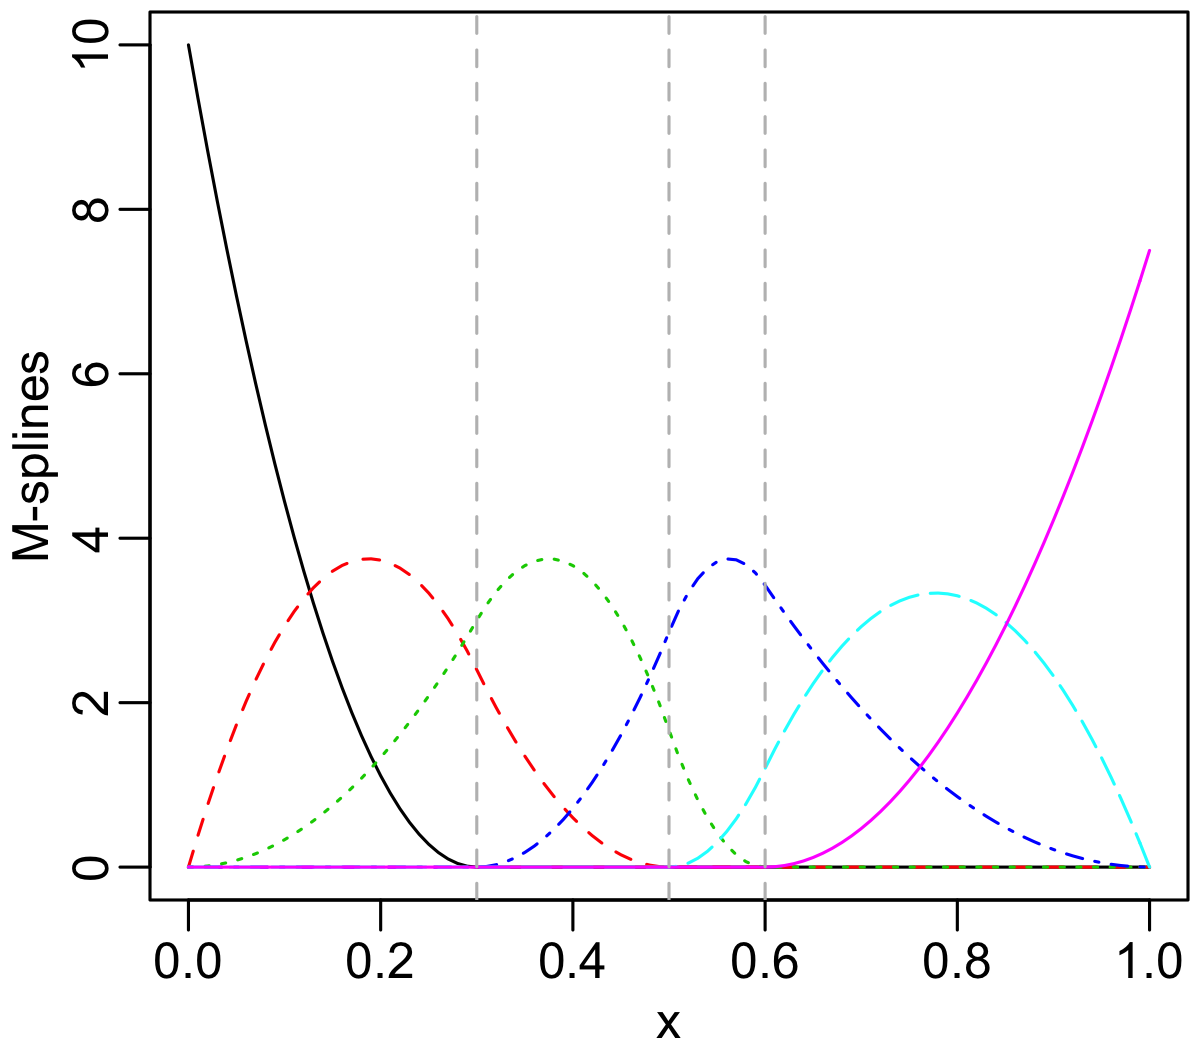
\includegraphics[width=0.45\linewidth]{figs/mSpline} 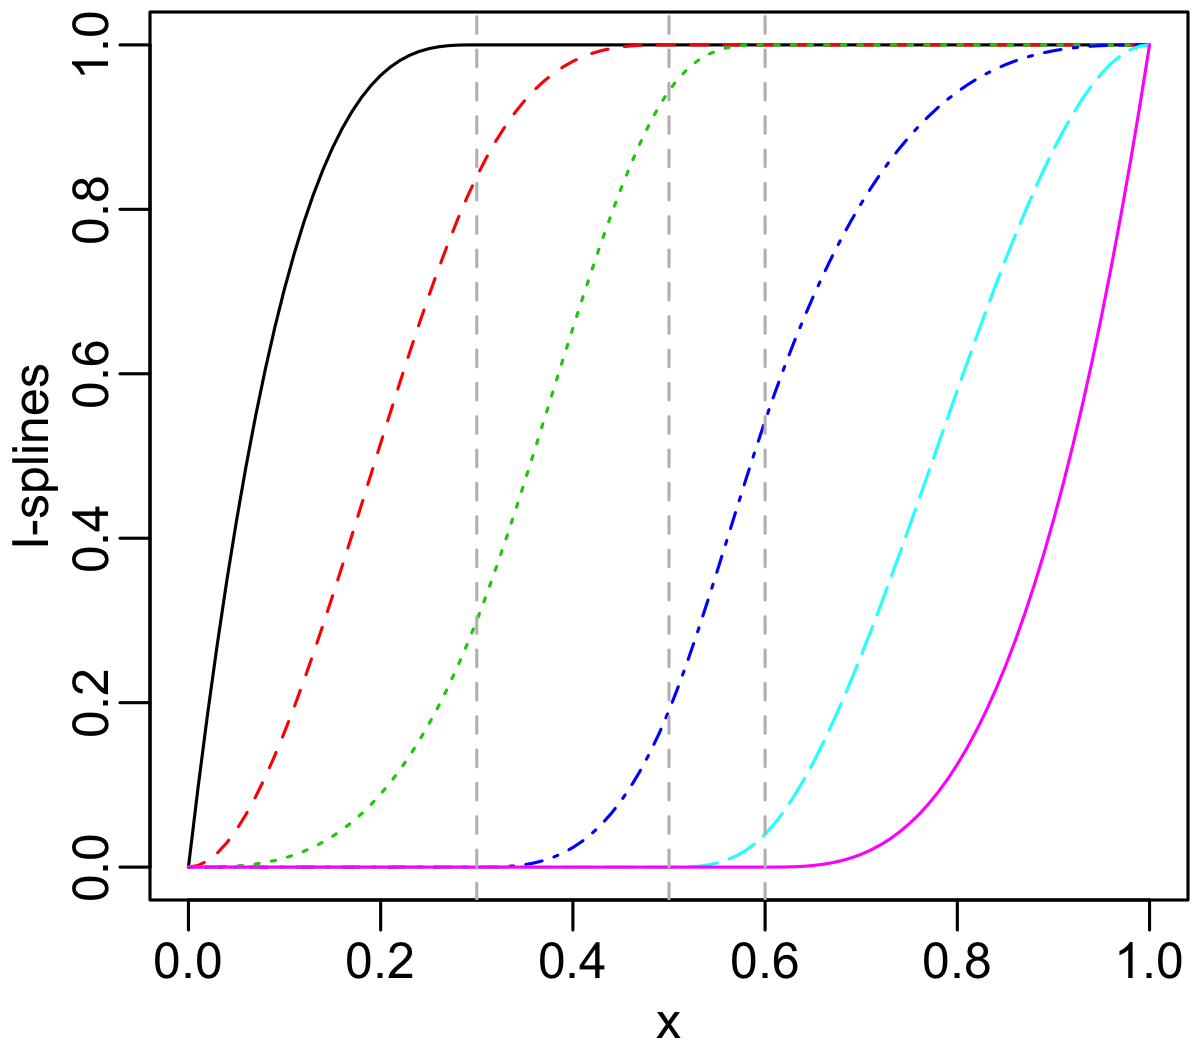
\includegraphics[width=0.45\linewidth]{figs/iSpline} 

}

\caption{Quadratic M-spline (left) and I-spline (right) Bases
with three internal knots.}\label{fig:miSplines}
\end{figure}

In the code chunk shown above, the chunk option
\texttt{out.width\ =\ \textquotesingle{}45\%\textquotesingle{}} and
\texttt{fig.show\ =\ \textquotesingle{}hold\textquotesingle{}} were set
so that the plots were placed side by side. We may set the chunk option
\texttt{echo\ =\ FALSE} so that the code chunk generating the plots are
excluded from the output. Also, the chunk option \texttt{cache} can be
set to be \texttt{TRUE} for time-consuming code chunks once the code
chunk is unlikely to be modified.

\hypertarget{sec:table}{%
\section{Tables and Other R objects}\label{sec:table}}

Tables can be similarly generated by a code chunk within the source
document. Table \ref{tab:theorem-envs} was, in fact, generated by
function \texttt{knitr::kable}. Another simple example of table
generation by \texttt{knitr::kable} is given in the following code
chunk. Table \ref{tab:iris} is the resulting table.



\begin{Shaded}
\begin{Highlighting}[]
\NormalTok{knitr}\OperatorTok{::}\KeywordTok{kable}\NormalTok{(}\KeywordTok{head}\NormalTok{(iris), }\DataTypeTok{booktabs =} \OtherTok{TRUE}\NormalTok{,}
             \DataTypeTok{caption =} \StringTok{'The first six rows of the iris dataset.'}\NormalTok{)}
\end{Highlighting}
\end{Shaded}

\begin{table}

\caption{\label{tab:iris}The first six rows of the iris dataset.}
\centering
\begin{tabular}[t]{rrrrl}
\toprule
Sepal.Length & Sepal.Width & Petal.Length & Petal.Width & Species\\
\midrule
5.1 & 3.5 & 1.4 & 0.2 & setosa\\
4.9 & 3.0 & 1.4 & 0.2 & setosa\\
4.7 & 3.2 & 1.3 & 0.2 & setosa\\
4.6 & 3.1 & 1.5 & 0.2 & setosa\\
5.0 & 3.6 & 1.4 & 0.2 & setosa\\
5.4 & 3.9 & 1.7 & 0.4 & setosa\\
\bottomrule
\end{tabular}
\end{table}

There are other \proglang{R} packages that can be of tremendous help in
generating the \proglang{Markdown} source for various \proglang{R}
objects. For example, the package \pkg{xtable} \citep{dahl2016xtable}
provides a more sophisticated support for generation of table source for
\LaTeX~and HTML; the package \pkg{pander} \citep{daroczi2015pander}
provides functions for printing a variety of \proglang{R} objects in
\pkg{pandoc}'s \proglang{Markdown}; the package \pkg{stargazer}
\citep{hlavac2015stargazer} produces \LaTeX~code, HTML code and SCII
text for well-formatted tables for results from regression models. See
\href{https://cran.r-project.org/web/views/ReproducibleResearch.html}{CRAN
task view} on reproducible research for a more comprehensive package
list.

\hypertarget{sec:code}{%
\section{Code Chunk}\label{sec:code}}

In addition to \proglang{R}, the code chunk can be written in a variety
of other languages, such as \proglang{Bash}, \proglang{Python},
\proglang{SAS}, etc., by specifying the chunk option \texttt{engine}.
The following code chunk is one toy example written in
\proglang{Python 3}.

\begin{Shaded}
\begin{Highlighting}[]
\NormalTok{foo }\OperatorTok{=} \StringTok{"Hello "} \OperatorTok{+} \StringTok{"world!"}
\BuiltInTok{print}\NormalTok{(}\StringTok{"The length of '}\SpecialCharTok{%s}\StringTok{' is }\SpecialCharTok\NormalTok{ (foo, }\BuiltInTok{len}\NormalTok{(foo)))}
\end{Highlighting}
\end{Shaded}

\begin{Shaded}
\begin{Highlighting}[]
\OperatorTok{>>>}\NormalTok{  The length of }\StringTok{'Hello world!'} \KeywordTok{is} \FloatTok{12.}
\end{Highlighting}
\end{Shaded}

We may set the chunk option \texttt{eval\ =\ FALSE} if we only want to
present the code without evaluation.

\hypertarget{sec:widgets}{%
\section{HTML Widgets}\label{sec:widgets}}

The \pkg{htmlwidgets} package \citep{vaidyanathan2016htmlwidgets}
provides a framework for easily creating \proglang{R} bindings to
\proglang{JavaScript} libraries. Several \proglang{R} packages built
based on it, such as \pkg{leaflet} \citep{cheng2016leaflet} and \pkg{DT}
\citep{xie2016dt}, enable us to embed interactive HTML widgets in the
HTML output. For PDF output, a screenshot taken by the package
\pkg{webshot} \citep{chang2016webshot} will be included instead.

For example, we embed a map for the location of Department of Statistics
at University of Connecticut (UConn) by \pkg{leaflet} in Figure
\ref{fig:mapPdf}.



\begin{Shaded}
\begin{Highlighting}[]
\NormalTok{urlTemplate <-}\StringTok{ "https://\{s\}.tile.openstreetmap.org/\{z\}/\{x\}/\{y\}.png"}
\KeywordTok{leaflet}\NormalTok{(}\DataTypeTok{width =} \DecValTok{900}\NormalTok{, }\DataTypeTok{height =} \DecValTok{500}\NormalTok{) }\OperatorTok\StringTok{ }\KeywordTok{addTiles}\NormalTok{(}\DataTypeTok{urlTemplate =}\NormalTok{ urlTemplate) }\OperatorTok
\StringTok{    }\KeywordTok{setView}\NormalTok{(}\OperatorTok{-}\StringTok{ }\FloatTok{72.251113}\NormalTok{, }\FloatTok{41.810757}\NormalTok{, }\DataTypeTok{zoom =} \DecValTok{17}\NormalTok{) }\OperatorTok
\StringTok{    }\KeywordTok{addPopups}\NormalTok{(}\OperatorTok{-}\StringTok{ }\FloatTok{72.251113}\NormalTok{, }\FloatTok{41.810757}\NormalTok{,}
              \StringTok{'<b>Department of Statistics, UConn</b>'}\NormalTok{)}
\end{Highlighting}
\end{Shaded}

\begin{figure}

{\centering 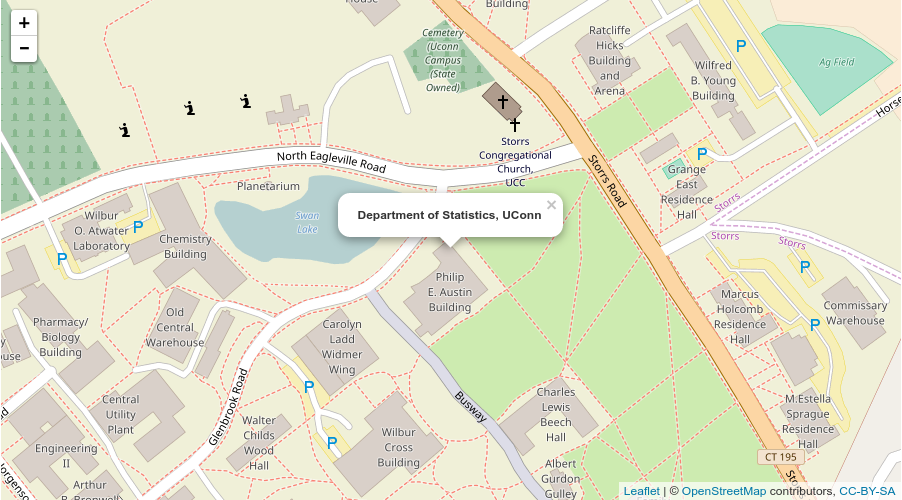
\includegraphics[width=0.9\linewidth]{figs/webshot_mapUConn} 

}

\caption{A map widget rendered via the \pkg{leaflet} package.}\label{fig:mapPdf}
\end{figure}

Another example of using the package \pkg{DT} to display \texttt{mtcars}
data is given here. The result is shown in Figure \ref{fig:dtPdf}.



\begin{Shaded}
\begin{Highlighting}[]
\NormalTok{DT}\OperatorTok{::}\KeywordTok{datatable}\NormalTok{(mtcars)}
\end{Highlighting}
\end{Shaded}

\begin{figure}

{\centering 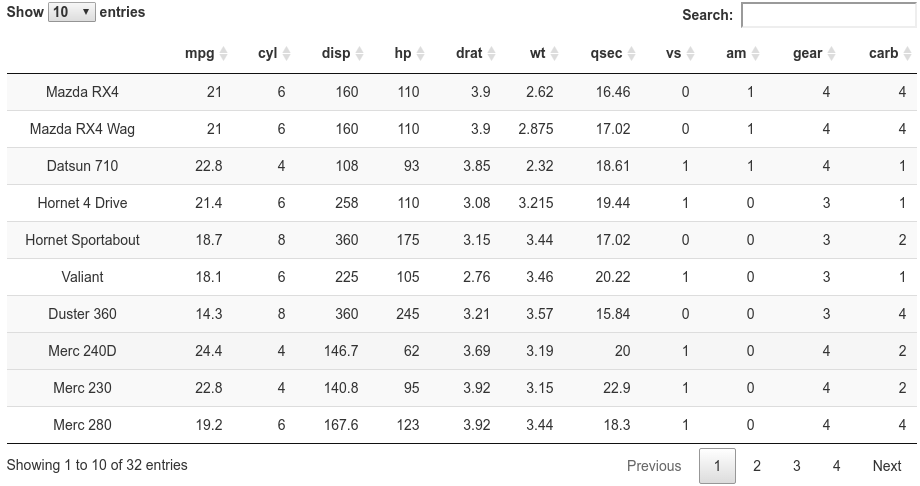
\includegraphics[width=0.9\linewidth]{figs/webshot_mtcars} 

}

\caption{A table widget rendered via the \pkg{DT} package.}\label{fig:dtPdf}
\end{figure}

\hypertarget{sec:shiny}{%
\section{Shiny Apps}\label{sec:shiny}}

The package \pkg{shiny} \citep{chang2017shiny} is a great tool providing
readers with an interactive way to explore data and results. We may
easily build Shiny applications on our own, deploy, and share it online
at \href{https://www.shinyapps.io/}{shinyapps.io} by the package
\pkg{rsconnect} \citep{allaire2016rsconnect}. In addition to building
regular applications by \pkg{Shiny}, the package \pkg{miniUI}
\citep{cheng2016miniUI} provides layout function designed for Shiny
applications with appropriate size on small screens.

We may embed Shiny applications in the document by
\texttt{knitr::include\_app}, which is mainly designed for HTML output.
Similarly, a screenshot taken by \pkg{webshot} will be embedded instead
for PDF output. The package \pkg{webshot} provides argument
\texttt{zoom} for a possible high resolution screenshot. However, if the
resolution is still not satisfactory, we may take a screenshot and
include it manually by \texttt{knitr::include\_graphics}.

An example Shiny application visualizing different kind of spline bases
is given in Figure \ref{fig:miniappPdf}.




\begin{Shaded}
\begin{Highlighting}[]
\NormalTok{knitr}\OperatorTok{::}\KeywordTok{include_app}\NormalTok{(}\StringTok{"https://wenjie-stat.shinyapps.io/minisplines2/"}\NormalTok{, }\StringTok{"500px"}\NormalTok{)}
\end{Highlighting}
\end{Shaded}

\begin{figure}

{\centering 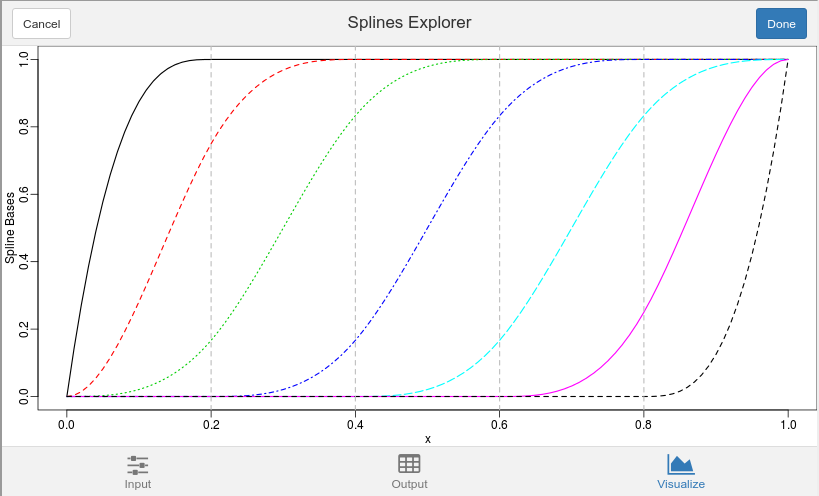
\includegraphics[width=0.9\linewidth]{figs/webshot_miniSplines2} 

}

\caption{An example of Shiny app visualizing different spline
bases available at \url{https://wenjie-stat.shinyapps.io/minisplines2}.}\label{fig:miniappPdf}
\end{figure}

\hypertarget{sec:summary}{%
\section{Summary and Discussion}\label{sec:summary}}

In summary, we provided this project template and reviewed most common
components and their syntax of writing a single \proglang{R Markdown}
document with the power and love of \pkg{bookdown} and many other
fantastic packages.

\citet{xie2017bookdown} provided a thorough introduction to
\pkg{bookdown} including more advanced customization and other output
formats. Additionally, the \href{http://pandoc.org/MANUAL.html}{manual}
of \pkg{Pandoc} gives all the available options that can be specified
through the \proglang{YAML} metadata section.

The template source and other associated files, such as BibTeX and CSS
file, are available at our GitHub repository \emph{dslab-templates}:
\url{https://github.com/statds/dslab-templates}.

\hypertarget{acknowledgment}{%
\section*{Acknowledgment}\label{acknowledgment}}
\addcontentsline{toc}{section}{Acknowledgment}

We would like to thank Yihui Xie and all the other authors and
contributors for the fabulous \pkg{knitr}, \pkg{rmarkdown}, and
\pkg{bookdown} packages. It would also be impossible for this template
to work without the fantastic open-source software: \proglang{R},
\pkg{pandoc}, etc.

\renewcommand\refname{Reference}
\bibliography{template.bib}

% not used now


\end{document}
